% Findings filed 24 November 2026 (report version 2.2)
\section{Detailed findings filed in this version (24 November 2026)}

This round targeted engineering results rather than input handling or reporting: a load-path audit of the dead-load combination, an AST sweep of the whole source for one operator-precedence bug class, and consistency oracles on the design checks (the same design shear strength in every check; the area, lever arm and inertia of a shear-flow formula all taken from the same section). Each finding was reproduced in at least two fresh processes and proven with a test-only monkeypatch. All upstream issues, by then numbered to \issue{310}, were screened for duplicates first.

% ---- 312
\subsection{\issue{312} --- Superimposed dead loads never enter the DL combination}
\textbf{Severity / tier:} \sevH\ candidate / T1. \quad \textbf{Proof:} \proof{312\_sidl\_missing\_from\_dead\_load\_combination/}

\textbf{Description.} \texttt{create\_dead\_load\_combination()} (\texttt{analyser.py:1516}) builds \texttt{DL} from four sub-cases, the fourth being \texttt{sidl\_combination} --- crash barrier, railing and median (\texttt{\_DL\_ATTRS}, \texttt{:1532--1537}). \texttt{create\_sidl\_combination()} (\texttt{:1564}) is \emph{never called anywhere in the code base}, so that entry is always \texttt{None} and is silently skipped. Every combination maps \texttt{'dead\_load'} to this case (\texttt{:2319}, \texttt{:2517}), as does the seismic mass (\texttt{:1040}). The loads are still applied to the grillage and still appear in the report's quantities, which hides the omission.

\begin{center}\begin{tabular}{@{}lrr@{}}
\toprule
Span 20\,m, no footpath, no median & As shipped & With SIDL in DL \\
\midrule
\texttt{crash\_barrier\_load\_case} & 261.6\,kN (applied, unused) & 261.6\,kN \\
\texttt{dead\_load\_combination} & 1160.4\,kN (= 97.9 + 1062.5 exactly) & 1422.0\,kN \\
Design moment $M_u$ & 1141.82\,kNm & 1211.25\,kNm \\
Design shear $V_u$ & 250.02\,kN & 266.17\,kN \\
Seismic dead-load mass & 1364.4\,kN & 1626.0\,kN \\
\bottomrule
\end{tabular}\end{center}

With footpath and median the excluded load is 400.5\,kN. Every girder check is under-stated: moment $+6.1$\,\%, shear $+6.5$\,\%, construction LTB $+14.4$\,\%, deflection $+6.7$\,\%, fatigue stress $+6.4$\,\%.

\begin{figure}[H]\centering
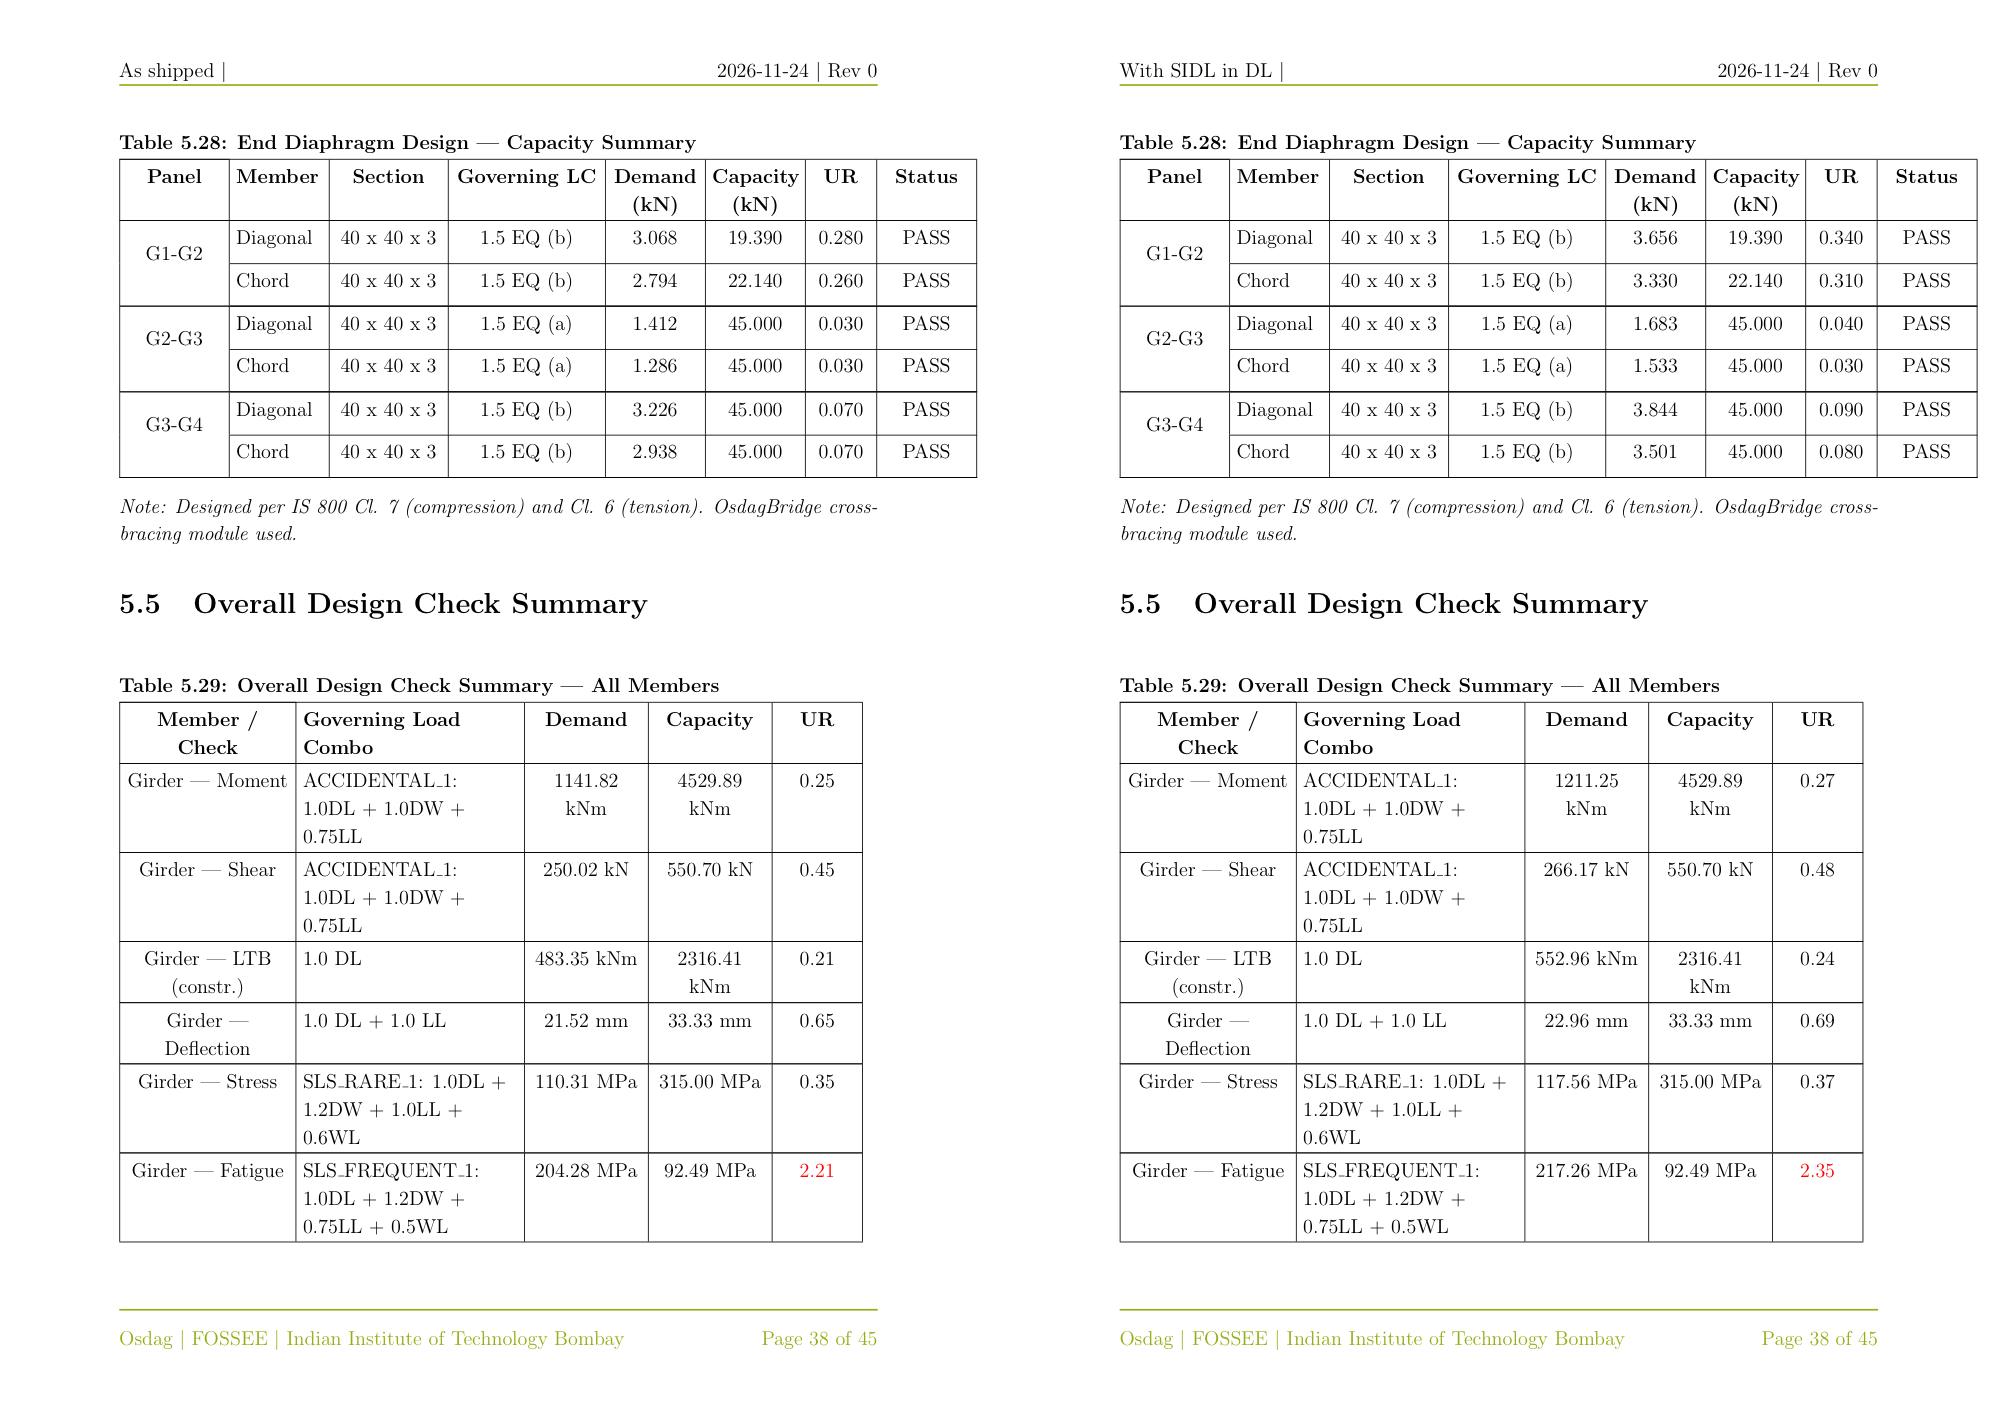
\includegraphics[width=0.92\linewidth]{../proofs/312_sidl_missing_from_dead_load_combination/screenshots/overall_summary_shipped_vs_sidl_fixed.png}
\caption{Overall Design Check Summary from OsdagBridge's own report: as shipped (left) and with the single missing call added (right).}
\end{figure}

% ---- 313
\subsection{\issue{313} --- \texttt{beta\_b} is always 1.0}
\textbf{Severity / tier:} \sevM\ / T1. \quad \textbf{Proof:} \proof{313\_beta\_b\_precedence\_plastic\_moment/}

\textbf{Description.} \texttt{beta\_b = 1.0 if section\_class == KEY\_Plastic or KEY\_Compact else Ze/Zp} parses as \texttt{(section\_class == KEY\_Plastic) or KEY\_Compact}. \texttt{KEY\_Compact} is the non-empty string \texttt{"Compact"}, so the condition is always true and the \texttt{Ze/Zp} branch is dead code. All five class names return the same 2664.22\,kNm; the correct value for the tested girder is 2371.60\,kNm. The program classifies that girder as \textbf{Slender} itself ($d/t_w = 136.0$ against a limit of 106.49) and still applies the plastic modulus.

The executed copy lives in the \texttt{osdag\_core} dependency (\texttt{is800\_2007.py:1012}), which \texttt{irc22\_2015.py:9--11} prefers over OsdagBridge's identical bundled copy (\texttt{:1026}). \texttt{irc22\_2015.py:649} returns $\chi_{LT}\cdot M_{pl}$, so the unreduced value reaches the check; the correct \texttt{beta\_b} that IRC22 computes at \texttt{:626--628} is used only for $\lambda_{LT}$.

\textbf{Effect:} LTB capacity overstated by $Z_p/Z_e = 12.3$\,\% --- construction-stage $M_b$ 2316.41 against 2062.00\,kNm. A side effect is that the section classification the program prints has no influence at all on the bending resistance.

% ---- 315
\subsection{\issue{315} --- M-V interaction fed the plastic shear capacity}
\textbf{Severity / tier:} \sevM\ / T1. \quad \textbf{Proof:} \proof{315\_mv\_interaction\_uses\_plastic\_shear/}

\textbf{Description.} IRC 22 Cl.\,603.3.3.3 reduces the bending strength when $V > 0.6\,V_d$, with $V_d$ the governing design shear strength. The code computes the plastic capacity (\texttt{designer.py:1762}) and the shear buckling resistance (\texttt{:1785}), uses the buckling value for the shear check and the report, and then passes the \emph{plastic} value to the interaction (\texttt{:1826}).

\begin{center}\begin{tabular}{@{}lrr@{}}
\toprule
Span 25\,m, carriageway 7.5\,m, median & As shipped & Governing $V_d$ \\
\midrule
$V_u$ / $V_{cr}$ (buckling) & 334.56 / 443.02\,kN & same \\
High-shear threshold $0.6\,V_d$ & 1193.9\,kN & 265.8\,kN \\
$\beta$ & 0.0 & 0.2605 \\
$M_{dv}$ & 7022.18\,kNm & 6052.79\,kNm \\
\bottomrule
\end{tabular}\end{center}

The capacity is 13.8\,\% too high. A hand check (IS 800 Cl.\,9.2.2, $M_{fd} = 3300.3$\,kNm) gives 6052.8\,kNm, matching the patched run. In a sweep of 20 designs, \textbf{six} fall in the window $0.6\,V_{cr} < V_u < 0.6\,V_d$ where the reduction is skipped.

\begin{figure}[H]\centering
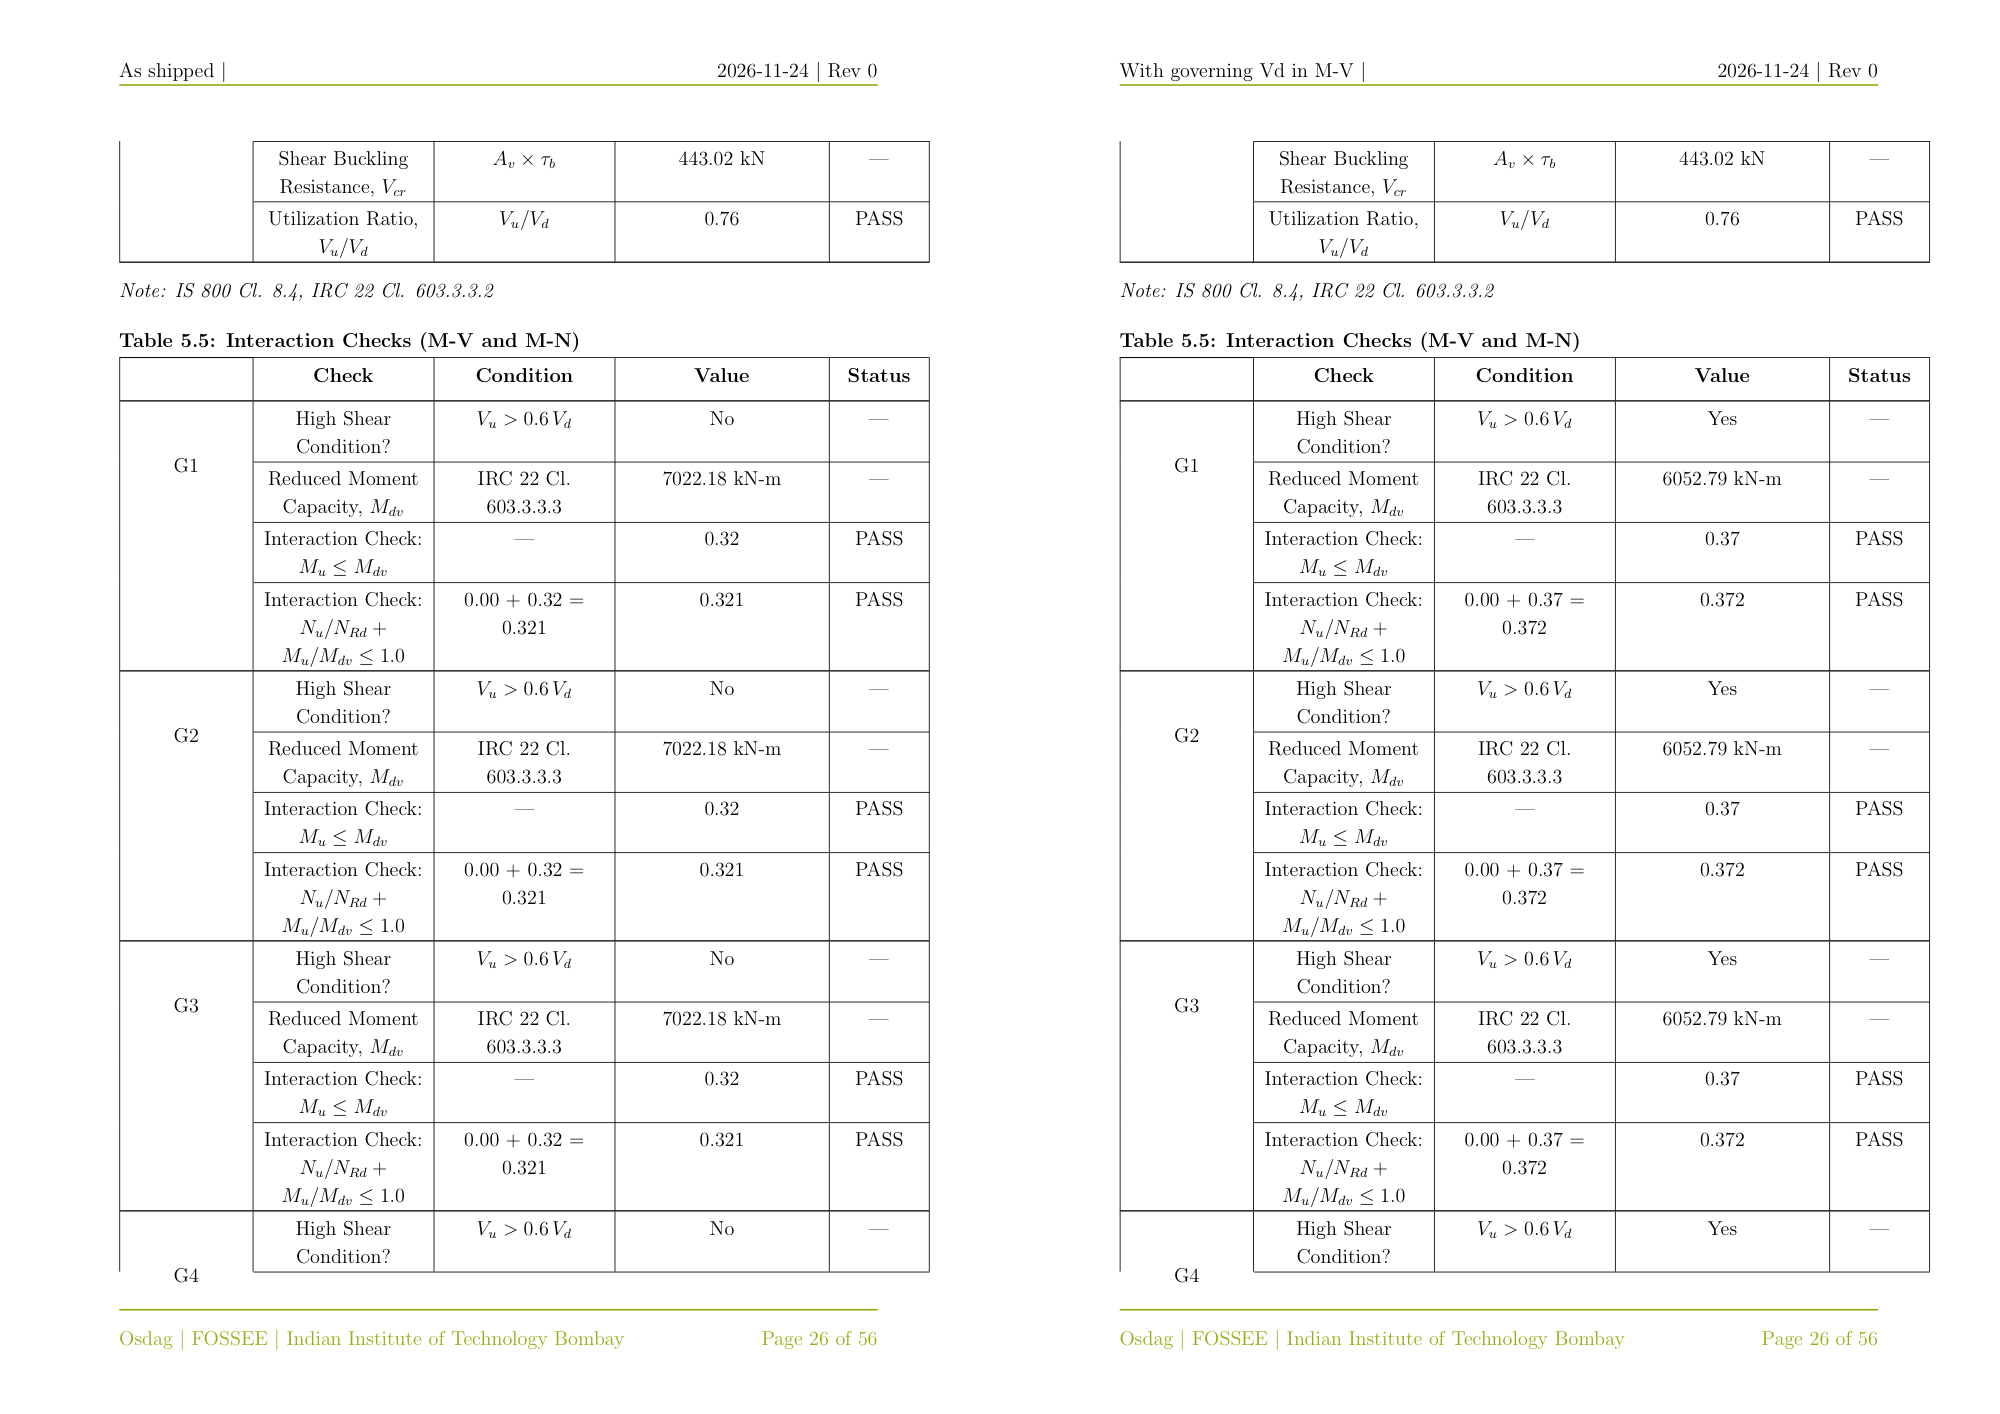
\includegraphics[width=0.92\linewidth]{../proofs/315_mv_interaction_uses_plastic_shear/screenshots/interaction_table_shipped_vs_governing_Vd.png}
\caption{Report page 26: the same page prints the shear utilisation $V_u/V_d = 0.76$ PASS and, directly below, ``High Shear Condition? $V_u > 0.6V_d$ --- No''. Right: with the governing $V_d$.}
\end{figure}

% ---- 316
\subsection{\issue{316} --- Longitudinal shear mixes plastic and elastic section properties}
\textbf{Severity / tier:} \sevM\ / T1. \quad \textbf{Proof:} \proof{316\_longitudinal\_shear\_plastic\_vs\_elastic\_na/}

\textbf{Description.} \texttt{irc22\_2015.py:1776} evaluates the elastic shear-flow formula $V_L = V\,A\,\bar{y}/I$, but takes $\bar{y}$ about the \emph{plastic} neutral-axis depth $x_u$ (\texttt{:1766}) while dividing by the \emph{elastic} composite inertia, and uses $n = E_s/E_{cm} = 6.061$ (\texttt{:1757}) instead of the IRC 22 Cl.\,604.3 floor of 7.5 that the inertia was built with. For the 20\,m case $x_u = 207.6$\,mm while the elastic neutral axis --- which the program reports itself as \texttt{y\_top\_comp\_mm} --- is at 274.7\,mm.

\textbf{Effect:} $V_L$ = 116.913 instead of 164.136\,N/mm, i.e.\ 28.8\,\% low. $V_L$ also feeds the deck transverse-shear check (\texttt{designer.py:1950--1951}), so the required transverse reinforcement is reported as 0.585 instead of 0.821\,cm$^2$/m. The provided stud spacing is unchanged here because the full-shear-connection criterion governs.

\paragraph{Duplicates confirmed in this round.} Two further leads were measured but already reported upstream: \issue{134} (footpath + median gives NaN load effects, zero demands and a wrong PASS) and \issue{257} (end diaphragms never designed at skew $0^\circ$). An AST sweep of the whole OsdagBridge source for the \texttt{x == A or B} precedence pattern found no instance other than \issue{313}.

\paragraph{Checked and found correct.} Girder section properties ($A$, $I_z$, $Z_e$, $Z_p$ all exact against hand calculation), the shear capacities and $K_v$ / $\tau_b$, $N_{Rd}$, the effective width $b_{eff} = \min(L/4,\ \mathrm{spacing})$, the deflection limits $L/800$ and $L/600$, and the composite modular ratios 7.5 / 15.0 (the IRC 22 Cl.\,604.3 minima, not a hard-coded error).
